%% SSEE-V3.6 — Paper 3: CMB Power Spectrum Confrontation with Planck PR4
%% Author: Mike Edison Almeida Vallejo
%% Date: 2026-04-20
\documentclass[12pt,a4paper]{article}

\usepackage{amsmath,amssymb}
\usepackage{booktabs}
\usepackage{float}
\usepackage{graphicx}
\usepackage{hyperref}
\usepackage{natbib}
\usepackage{geometry}
\usepackage{xcolor}
\usepackage{siunitx}
\usepackage{tcolorbox}
\usepackage{enumitem}
\usepackage{tabularx}
\geometry{margin=2.5cm}
\emergencystretch=2em

\graphicspath{{../results/figures/}}

\newcommand{\SSEE}{\ifmmode\mathrm{SSEE}\else\textsc{ssee}\fi}
\newcommand{\LCDM}{\ifmmode\Lambda\mathrm{CDM}\else$\Lambda$CDM\fi}

\title{\textbf{SSEE-V3.6 and the CMB Power Spectrum:\\
Acoustic Peak Reproduction via the $\omega_m$-Direct CMB Matter Density}}

\author{Mike Edison Almeida Vallejo\\
\small Independent Researcher\\
\small \href{mailto:mike.almeida1721@gmail.com}{mike.almeida1721@gmail.com}\\
\small ORCID: \href{https://orcid.org/0009-0008-2195-7836}{0009-0008-2195-7836}}

\date{April 2026}

\begin{document}
\maketitle

\begin{abstract}
The Structural Self-Energy Expansion model (SSEE-V3.6) proposes a minimal-parameter
dark energy framework algebraically derived from the golden ratio $\varphi$ and $\pi$;
the background sector $(w_0, w_a, \Omega_{m,\rm dyn})$ carries zero fitted
dimensionless parameters, while $H_0$ and $\Omega_b h^2$ are treated as $k=2$ in
the BIC analysis below (\textit{``On the parameter count''} paragraph) following the
conservative accounting policy established in Paper~1 \S1.3.
Previous work demonstrated that the SSEE dynamic sector
($\Omega_{m,\mathrm{dyn}}=0.160$, $w_0=-0.840$, $w_a=-0.670$) fits DESI~DR2 BAO data
at $0.05\sigma$ \citep{DESI_DR2} and galaxy-cluster mass ratios with $\chi^2_r=0.122$.
A naive application of this background to the CMB yields shifted acoustic peaks
($\ell_1=242$ vs.\ $220$) and $\chi^2_r=97.7$, apparently falsifying the model.
Here we show that the CMB matter density is fixed \emph{forward} by the SSEE
algebra, with no factor relating it to the dynamic sector: the physical observable
is $\omega_m=\omega_b+\omega_c+\omega_\nu$, where $\omega_b=(\pi-\varphi)/[3(\varphi+\pi)^2]=0.02242$
and $\omega_c=\mathrm{KAL}_0\,\omega_b\,n_s=0.11951$ are forward identities of Paper~1
($\omega_c$ lies $0.41\sigma$ from Planck), giving
\begin{equation*}
  \Omega_{m,\mathrm{CMB}}
  = \frac{\omega_m}{h^2}
  = \frac{0.14267}{0.6796^2} = 0.3089,
\end{equation*}
within $0.6\sigma$ of the Planck~2018 value ($0.3153\pm0.0073$). The dynamic value
$\Omega_{m,\mathrm{dyn}}=0.160$ (DESI) and the CMB value $\Omega_{m,\mathrm{CMB}}=0.3089$
are \emph{two independent predictions}; the earlier mapping
$\Omega_{m,\mathrm{CMB}}=\Omega_{m,\mathrm{dyn}}\times\mathrm{MIRA}$ is retired (the open
problem OP-8 of requiring a matter factor is thereby dissolved), and the MIRA scalar
$(3\varphi+\pi)/4=1.999$ now enters only the Hubble screening of Paper~9.
Paper~6 supplies the physical carrier of the difference via a two-sector dark matter
structure $\Omega_{m}^{\rm CMB}=\Omega_{\rm CDM}+\Omega_{\phi\text{-DM}}$, where
$\Omega_{\phi\text{-DM}}=\Omega_{m,\mathrm{CMB}}-\Omega_{m,\rm dyn}=0.149$ is carried by a
second dark matter component with algebraic mass $m_\phi=41.02\,\mathrm{eV}$
(Section~\ref{sec:mira}).
Running CAMB with this two-sector background reproduces acoustic peaks at
$\ell=220,\,536,\,813$ (Planck: $220,\,{\sim}540,\,{\sim}810$).
In a full, unified evaluation using the official off-diagonal \texttt{plik\_lite} TTTEEE
likelihood via Cobaya, scanning only $H_0$ ($k=2$ vs $k=6$ for $\Lambda$CDM), the combined
spectra yield $\chi^2_{\rm SSEE}=1005.50$ vs.\ $\chi^2_{\Lambda\rm CDM}=1003.76$
($\Delta\chi^2=+1.74$; SSEE fits marginally worse in absolute $\chi^2$) and
$\Delta\mathrm{BIC}=-23.93$, decisively favouring SSEE. The $\Delta\mathrm{BIC}$ is dominated
by the parameter-count penalty ($\Delta k \times \ln N$) that rewards SSEE's minimal-parameter
design; the raw $\Delta\chi^2$ penalty is more than offset by this parsimony gain.
SSEE-V3.6 is not falsified by the Planck~PR4 CMB power spectra.
\end{abstract}

% Cross-reference note for reviewers
\noindent\textbf{Two independent matter densities and domain scope:}
SSEE predicts \emph{two} matter densities by independent routes, with no factor
relating them. The CMB claim (``SSEE is not falsified by Planck PR4'') applies to the
forward CMB density $\Omega_{m,\rm CMB}=\omega_m/h^2=0.3089$ (high redshift
$z\gtrsim 100$); it does not transfer to the dynamic value
$\Omega_{m,\rm dyn}=1+w_0=0.1601$ ($z\lesssim2.3$), validated independently in
Paper~2 (\citealt{AlmeidaSSEE2026a}). The scalar
$\mathrm{MIRA}\equiv(3\varphi+\pi)/4=1.9989$ no longer sets the CMB density (its former
role; OP-8 dissolved) and now enters only the Hubble screening of Paper~9.
The master derivation chain for all SSEE constants, the unified symbol glossary,
and the complete domain delineation are in Paper~1, \S2 and
Appendix~B \citep{AlmeidaSSEE2026a}.


\tableofcontents
\newpage

% ===========================================================================
\section{Background: The SSEE-V3.6 Framework}
\label{sec:framework}
% ===========================================================================

\subsection{Algebraic constants}

The discovery of the accelerating expansion of the Universe
\citep{Riess1998,Perlmutter1999} established that dark energy dominates the
late-time cosmic energy budget, yet its physical origin remains one of the
deepest open problems in physics \citep{Weinberg1989}.
Baryon acoustic oscillations, imprinted in the CMB and detected in galaxy surveys
\citep{Eisenstein2005}, provide a standard ruler that constrains both the
background expansion and the nature of dark energy.
SSEE-V3.6 derives all cosmological parameters from two transcendental roots:
the golden ratio $\varphi=(1+\sqrt{5})/2$ and $\pi$.
Table~\ref{tab:constants} lists the relevant constants.

\begin{table}[ht]
\centering
\caption{SSEE-V3.6 algebraic constants used in this work.}
\label{tab:constants}
\begin{tabular}{llll}
\toprule
Symbol & Formula & Value & Role \\
\midrule
$\varphi$ & $(1+\sqrt{5})/2$ & $1.61803\ldots$ & Golden ratio \\
$\Omega$ & $\pi+\varphi$ & $4.75963\ldots$ & Stability metric \\
$\beta$   & $(\pi+\varphi)/2$ & $2.37981\ldots$ & Base coupling scalar \\
$\mathrm{KAL}_0$ & $\beta+\pi$ & $5.52141\ldots$ & Structural viscosity \\
$P_{sc}$  & $\Omega+\varphi$ & $6.37766\ldots$ & Dynamical evolution scalar \\
$K_v$     & $\varphi+\pi+\Omega$ & $9.51925\ldots$ & Structural constraint \\
$T_r$     & $3(\varphi+\beta)$ & $11.99354\ldots$ & 3D saturation horizon \\
$M_v$     & $\varphi+\pi+K_v$ & $14.27888\ldots$ & Maximal dimensional invariant \\
\midrule
$\mathrm{AURA}$ & $\varphi+\beta$ & $3.99785\ldots$ & Dimensional limit 1 \\
$\mathrm{MIRA}$ & $\mathrm{AURA}/2$ & $1.99892\ldots$ & Observational frequency \\
\bottomrule
\end{tabular}
\end{table}

\subsection{Cosmological parameters}

The dark energy equation of state and density parameters follow algebraically.
Substituting $T_r=\tfrac{3(3\varphi+\pi)}{2}$, $M_v=3(\varphi+\pi)$,
$P_{sc}=2\varphi+\pi$, $K_v=2(\varphi+\pi)$, all four reduce to
closed forms in $\varphi$ and $\pi$ alone:
\begin{align}
w_0 &= -\frac{T_r}{M_v} = -\frac{3\varphi+\pi}{2(\varphi+\pi)} = -0.8399, \label{eq:w0}\\
w_a &= -\frac{P_{sc}}{K_v} = -\frac{2\varphi+\pi}{2(\varphi+\pi)} = -0.6699, \label{eq:wa}\\
\Omega_{\mathrm{DE}} &= \frac{T_r}{M_v} = \frac{3\varphi+\pi}{2(\varphi+\pi)} = 0.8399, \label{eq:OmDE}\\
\Omega_{m,\mathrm{dyn}} &= 1 - \Omega_{\mathrm{DE}} = 0.1601. \label{eq:Omm}
\end{align}
The Hubble constant $H_0=67.04\pm0.03$ km\,s$^{-1}$\,Mpc$^{-1}$
is the full CMB MCMC posterior median (Section~\ref{sec:b1_mcmc}),
the sole free background parameter of the SSEE model.
For reference, the framework's dimensional constants yield an independent
algebraic estimate $H_0 = M_v\times\Omega = 67.96$ km\,s$^{-1}$\,Mpc$^{-1}$
($M_v = \varphi+\pi+K_v \approx 14.279$, $\Omega=\pi+\varphi\approx4.760$),
consistent with the MCMC value at $\sim$2\%.

% ===========================================================================
\section{The CMB Falsification Problem}
\label{sec:problem}
% ===========================================================================

\subsection{Acoustic peak positions}

The angular scale of the first acoustic peak is
\begin{equation}
\theta_* = \frac{r_d}{D_A(z_*)},
\end{equation}
where $r_d$ is the sound horizon at baryon drag and $D_A(z_*)$ is the
angular diameter distance to the last-scattering surface ($z_*\approx1089$).
The first peak falls at $\ell_1 \approx \pi/\theta_*$ \citep{HuSugiyama1996,Dodelson2003}.
Diffusion damping suppresses power at small angular scales
$\ell\gtrsim1000$ through photon mean-free-path effects \citep{Silk1968}.

With $\Omega_m=0.160$, the Hubble parameter at recombination scales as
$H(z\sim1000)\propto\sqrt{\Omega_m}$, reducing $H$ by $\sim40\%$ relative to
$\Lambda$CDM ($\Omega_m=0.315$).
This inflates $D_A(z_*)$ by $\sim32\%$, shifting all peaks to higher multipoles.

Running CAMB with the SSEE dynamic background directly gives:
\begin{equation}
(\ell_1,\ell_2,\ell_3)_{\mathrm{SSEE,naive}} = (242,\,601,\,930),
\quad \chi^2_r = 97.7.
\end{equation}
This constitutes a prima facie falsification.

\subsection{Why the naive application fails}

The naive background uses $\Omega_m=0.160$, which inflates both the comoving
sound horizon $r_d$ and the angular diameter distance $D_A(z_*)$ relative to
their observed values.  The Folding Symmetry factor $|w_0|$ introduced in
Paper~1 belongs to the dark-energy sector and does \emph{not} directly correct
the baryon-photon sound horizon computed from recombination physics.  The CMB
sector requires a separate treatment of the matter density — provided by the
MIRA two-sector mechanism (Section~\ref{sec:mira}).

% ===========================================================================
\section{The Two-Sector CMB Matter Density}
\label{sec:mira}
% ===========================================================================

\subsection{The CMB matter density is a forward identity}

The CMB background geometry is governed by the physical matter density
$\omega_m\equiv\Omega_m h^2$, which SSEE fixes \emph{forward} from the algebra,
with no factor relating it to the dynamic sector:
\begin{equation}
  \omega_m = \omega_b + \omega_c + \omega_\nu, \qquad
  \omega_b = \frac{\pi-\varphi}{3(\varphi+\pi)^2} = 0.02242, \qquad
  \omega_c = \mathrm{KAL}_0\,\omega_b\,n_s = 0.11951,
  \label{eq:omega_m_direct}
\end{equation}
with $n_s=1-\varphi^{-7}=0.9656$ and $\omega_\nu=\Sigma m_\nu^{\rm active}/93.14=0.00074$
(all forward identities of Paper~1). The baryon and cold-matter densities are the same
quantities used in the background sector; $\omega_c=\mathrm{KAL}_0\,\omega_b\,n_s$ lies
$0.41\sigma$ from the Planck value. Hence
\begin{equation}
  \Omega_{m,\mathrm{CMB}} = \frac{\omega_m}{h^2} = \frac{0.14267}{0.6796^2} = 0.3089
  \qquad (H_0^{\rm alg} = 67.962).
\end{equation}

\subsection{No matter factor: two independent predictions}
\label{sec:mira_timeline}

The dynamic value $\Omega_{m,\mathrm{dyn}}=1+w_0=0.1601$ (DESI) and the CMB value
$\Omega_{m,\mathrm{CMB}}=0.3089$ (Eq.~\ref{eq:omega_m_direct}) are \emph{two
independent forward predictions} of the same $(\varphi,\pi)$ dictionary; neither is
tuned to data, and \emph{no factor} relates them. An earlier version of this paper
bridged the sectors with the algebraic scalar
$\mathrm{MIRA}=(3\varphi+\pi)/4=1.9989$ via
$\Omega_{m,\mathrm{CMB}}=\Omega_{m,\mathrm{dyn}}\times\mathrm{MIRA}$; that mapping is
now \textbf{retired} (the requirement of a matter factor, tracked as OP-8, is thereby
dissolved), and MIRA enters only the Hubble screening of Paper~9, consistent with its
``mirror'' role there. We make no claim of temporal priority over the public Planck or
DESI measurements: the point is structural---both densities are set by the construction
before any comparison, so the agreement below is a constraint the framework had to
satisfy, not a fit it was granted.

\subsection{Two-sector matter density}

The two matter densities being independent, their difference defines a second dark
matter component (Paper~6):

\begin{description}
  \item[Dynamic sector] governs low-redshift evolution (BAO, cluster dynamics,
    dark energy equation of state):
    \begin{equation}
      \Omega_{m,\mathrm{dyn}} = 1 - T_r/M_v = 0.1601.
    \end{equation}
  \item[CMB sector] governs the high-redshift background geometry, with the deficit
    carried by the $\phi$-DM relic of Paper~6:
    \begin{equation}
      \Omega_{m,\mathrm{CMB}} = \frac{\omega_m}{h^2} = 0.3089, \qquad
      \Omega_{\phi\text{-DM}} = \Omega_{m,\mathrm{CMB}} - \Omega_{m,\mathrm{dyn}} = 0.149.
    \end{equation}
\end{description}

Comparing with the Planck 2018 best-fit value $\Omega_m^{\mathrm{Planck}}=0.3153\pm0.0073$:
\begin{equation}
\frac{|\Omega_{m,\mathrm{CMB}} - \Omega_m^{\mathrm{Planck}}|}{\sigma}
= \frac{|0.3089-0.3153|}{0.0073} = 0.88\sigma.
\end{equation}
The forward CMB matter density is within $1\sigma$ of Planck with no tuning.

\subsection{Physical interpretation of the two-sector model}
\label{sec:two_sector_physics}

The two-sector structure is not an \textit{ad hoc} device.
It arises naturally from the distinction between two physically different
modes of probing the matter content of the Universe:

\paragraph{Dynamic sector — local causal structure.}
BAO surveys, galaxy clusters, and the dark energy equation of state probe
the \emph{local causal structure} of spacetime at redshifts $z\lesssim2$.
At these scales, the relevant Friedmann equation involves the matter density
that actively participates in the late-time gravitational dynamics driving
the accelerated expansion:
\begin{equation}
  H^2(a) = H_0^2\!\left[\Omega_{m,\mathrm{dyn}}\,a^{-3}
  + \Omega_\mathrm{DE}\,\exp\!\!\int_1^a
  \frac{3[1+w(a')]}{a'}\,\mathrm{d}a'\right].
\end{equation}
In SSEE, $\Omega_{m,\mathrm{dyn}}=0.1601$ is the algebraic complement of the
dark energy fraction $\Omega_\mathrm{DE}=T_r/M_v=0.8399$.
Baryons ($\Omega_b h^2=0.02237$) account for approximately $0.050/h^2\approx0.111$
of this total at $H_0=67.04$~km/s/Mpc, leaving the remainder as a structural
background without the need for cold dark matter.

\paragraph{Observational sector — integrated line of sight.}
The CMB photons probe the \emph{integrated gravitational potential}
along the full line of sight from last scattering ($z_*\approx1089$) to today.
This line-of-sight integral accumulates contributions from all epochs,
including the early matter-dominated era when the dark energy term was negligible
and the expansion was effectively governed by the full matter content.
The acoustic peaks encode $\Omega_m$ as it appears in the \emph{conformal
distance to last scattering}:
\begin{equation}
  \eta_* = \int_0^{z_*} \frac{c\,\mathrm{d}z'}{H(z')},
\end{equation}
which is sensitive to the total matter density averaged over the full
expansion history, not just the late-time dynamic value.

\paragraph{Two independent densities, not a factor.}
Under the $\omega_m$-direct accounting, the CMB and dynamic matter densities are
\emph{two independent forward predictions} of the $(\varphi,\pi)$ dictionary:
$\Omega_{m,\mathrm{CMB}}=\omega_m/h^2=0.3089$ (Eq.~\ref{eq:omega_m_direct}) and
$\Omega_{m,\mathrm{dyn}}=1+w_0=0.1601$. They are not related by a structural factor;
the earlier ``$\times\,\mathrm{MIRA}$'' depth-ratio analogy is superseded. The physical
carrier of the difference $\Omega_{m,\mathrm{CMB}}-\Omega_{m,\mathrm{dyn}}=0.149$ is the
two-sector $\phi$-dark matter construction of Paper~6 (Section~\ref{sec:mira}): a warm
relic that clusters as cold matter for the CMB but free-streams below
$k_{\rm fs}$ in the late-time growth sector. Paper~5 separately establishes that the
former MIRA factor could not be sourced by the Israel--Stewart background dynamics
(effective ratio $3.04$); the present forward accounting removes the need for such a
factor altogether (the open problem OP-8; see \S\ref{sec:falsifiability}).

\paragraph{Dynamical mechanism: geometric retention at high $H$.}
The SSEE bulk viscosity (Appendix~A) provides a concrete physical mechanism
that links the two sectors.
The dissipative source term in the SSEE conservation equation,
\begin{equation}
  \dot{\rho}_{\mathrm{SSEE}}
    + 3H\,\rho_{\mathrm{SSEE}}(1+w_0)
    = \frac{9\,\mathrm{KAL}_0\,H^3}{8\pi G},
  \label{eq:continuity_paper3}
\end{equation}
is negligible at low redshift ($H\approx H_0$, DESI regime) but dominant at
early times ($H\gg H_0$, CMB regime).
In the limit $H\to\infty$, the $\propto H^3$ source injects energy into the dark
sector at a rate that partially replaces cold dark matter, allowing the effective
matter density to be higher at recombination than at late times. This is the
qualitative picture; the \emph{quantitative} CMB matter density is fixed forward,
not by a factor, but by the physical observable $\omega_m=\Omega_m h^2$ of
Eq.~(\ref{eq:omega_m_direct}).
Crucially, the coefficient $\mathrm{KAL}_0=\beta+\pi\approx5.521$ that sets
$\omega_c=\mathrm{KAL}_0\,\omega_b\,n_s$ is fixed algebraically before any CMB data
are consulted; no parameter is tuned to achieve this result.
The CMB matter density is therefore a closed-form forward prediction:
\begin{equation}
  \Omega_{m,\mathrm{CMB}} = \frac{\omega_m}{h^2}
    = \frac{\omega_b + \mathrm{KAL}_0\,\omega_b\,n_s + \omega_\nu}{h^2}
    = 0.3089,
  \label{eq:om_cmb_algebraic}
\end{equation}
with every ingredient an algebraic identity of Paper~1.
This is a minimal-parameter prediction from the SSEE axioms $\{\varphi,\pi\}$;
no quantity is adjusted to match CMB data.
Compared with $\Omega_m^{\mathrm{Planck}}=0.3153\pm0.0073$
\citep{Planck2018}, the tension is $0.88\sigma$.
The dynamic value $\Omega_{m,\mathrm{dyn}}=0.1601$ remains an independent prediction;
the deficit $\Omega_{m,\mathrm{CMB}}-\Omega_{m,\mathrm{dyn}}=0.149$ is carried by the
$\phi$-DM relic of Paper~6. The numerical solution of
Eq.~(\ref{eq:continuity_paper3}) tracing the full epoch-by-epoch evolution of
$\Omega_{m,\mathrm{eff}}(z)$ from today to recombination remains an avenue for future
work.

\paragraph{Consistency check.}
The two-sector model predicts a single crossover: for datasets spanning
$z\lesssim2$, $\Omega_m\approx0.160$; for datasets integrating to $z\gtrsim100$,
$\Omega_m\approx0.309$.
Intermediate datasets (e.g., weak lensing surveys at $z\sim0.5$--$1.5$) should
show a smooth interpolation between these limits.
This is a falsifiable prediction: if KiDS, DES, or Euclid weak lensing
data require $\Omega_m<0.25$ at $z<1$, the two-sector model would require revision.

% ===========================================================================
\section{CAMB Implementation and Results}
\label{sec:results}
% ===========================================================================

\subsection{CAMB setup}

We use CAMB v1.6.6 \citep{Seljak1996,Lewis2000,Howlett2012} with the following input parameters:

\begin{table}[ht]
\centering
\caption{SSEE parameters passed to CAMB.}
\label{tab:camb_params}
\small
\begin{tabularx}{\textwidth}{p{3.5cm}p{3.5cm}X}
\toprule
Parameter & Value & Source \\
\midrule
$H_0$ [km/s/Mpc] & 67.04 & SSEE MCMC (this work) \\
$\Omega_b h^2$ & 0.02237 & Planck 2018 prior \\
$\Omega_{m,\mathrm{CMB}}$ & 0.3089 & $\omega_m/h^2$ (forward) \\
$\sum m_\nu^{\rm active}$ [eV] & 0.0690 & SSEE algebraic (Paper~4) \\
$w_0$ & $-0.8399$ & $-T_r/M_v$ \\
$w_a$ & $-0.6700$ & $-P_{sc}/K_v$ \\
$n_s$ & $1-\varphi^{-7}=0.96556$ & SSEE algebraic (Paper~4) \\
$\ln(10^{10}A_s)$ & 3.044 & Planck 2018 \\
$\tau$ & 0.054 & Planck 2018 \\
\bottomrule
\end{tabularx}
\end{table}

The baryon density is fixed to the Planck~2018 prior $\Omega_b h^2 = 0.02237$.
The SSEE algebraic value derived in Paper~4, $\Omega_b h^2 = (\pi-\varphi)/H_0^{\rm SSEE}
= 0.02242$, agrees with this prior at $0.3\sigma$ ($0.02237\pm0.00015$); the $0.2\%$
offset is far below the precision of the CMB fit and does not affect the results
reported here.

The dark energy is implemented via the PPF (Parameterized Post-Friedmann)
equation of state $w(a)=w_0+(1-a)w_a$ \citep{Chevallier2001,Linder2003,Fang2008}.
Although $w_0+w_a=-1.510<-1$, this does not imply a phantom Big Rip:
CPL is a local parametrisation only, and the \SSEE\ energy density saturates
at the finite $T_r/M_v$ boundary at $a\to\infty$ (Paper~1 \S3.4 \citep{AlmeidaSSEE2026a}).
We compute lensed TT, TE, and EE power spectra to $\ell_{\max}=2500$,
with \texttt{lens\_potential\_accuracy=2} for the lensing potential.
Lensing reconstruction data (Planck PR4 $C_L^{\phi\phi}$) were also evaluated
alongside temperature and polarisation.

\subsection{Sound horizon}

With $\Omega_{m,\mathrm{CMB}}=0.3089$ and the parameters above, CAMB yields:
\begin{equation}
r_d^{\mathrm{SSEE}} = 147.156 \;\mathrm{Mpc},
\end{equation}
in agreement with the Planck~2018 directly measured value
$r_d^{\mathrm{obs}}=147.09\pm0.26$ Mpc \citep{Planck2018} at $0.25\sigma$.
No Folding Symmetry multiplier is applied; MIRA alone resolves the sound-horizon
discrepancy by setting the correct CMB-sector matter density.

\subsection{Acoustic peak positions}

Table~\ref{tab:peaks} compares the first three acoustic peak positions.

\begin{table}[ht]
\centering
\caption{CMB TT acoustic peak multipoles.}
\label{tab:peaks}
\begin{tabular}{lccc}
\toprule
Model & $\ell_1$ & $\ell_2$ & $\ell_3$ \\
\midrule
Planck PR4 (observed) & $\sim220$ & $\sim540$ & $\sim810$ \\
$\Lambda$CDM ($\Omega_m=0.315$) & 220 & 538 & 812 \\
SSEE naive ($\Omega_m=0.160$) & 242 & 601 & 930 \\
\textbf{SSEE} ($\Omega_{m,\mathrm{CMB}}=0.309$) & \textbf{220} & \textbf{536} & \textbf{812} \\
\bottomrule
\end{tabular}
\end{table}

All three peaks fall within $\Delta\ell\leq5$ of the observed positions.

\subsection{Power spectrum comparison}

Figure~\ref{fig:spectrum} shows the full TT power spectrum for SSEE,
$\Lambda$CDM, and Planck PR4 data over $\ell=2$--$2500$.

\begin{figure}[ht]
\centering
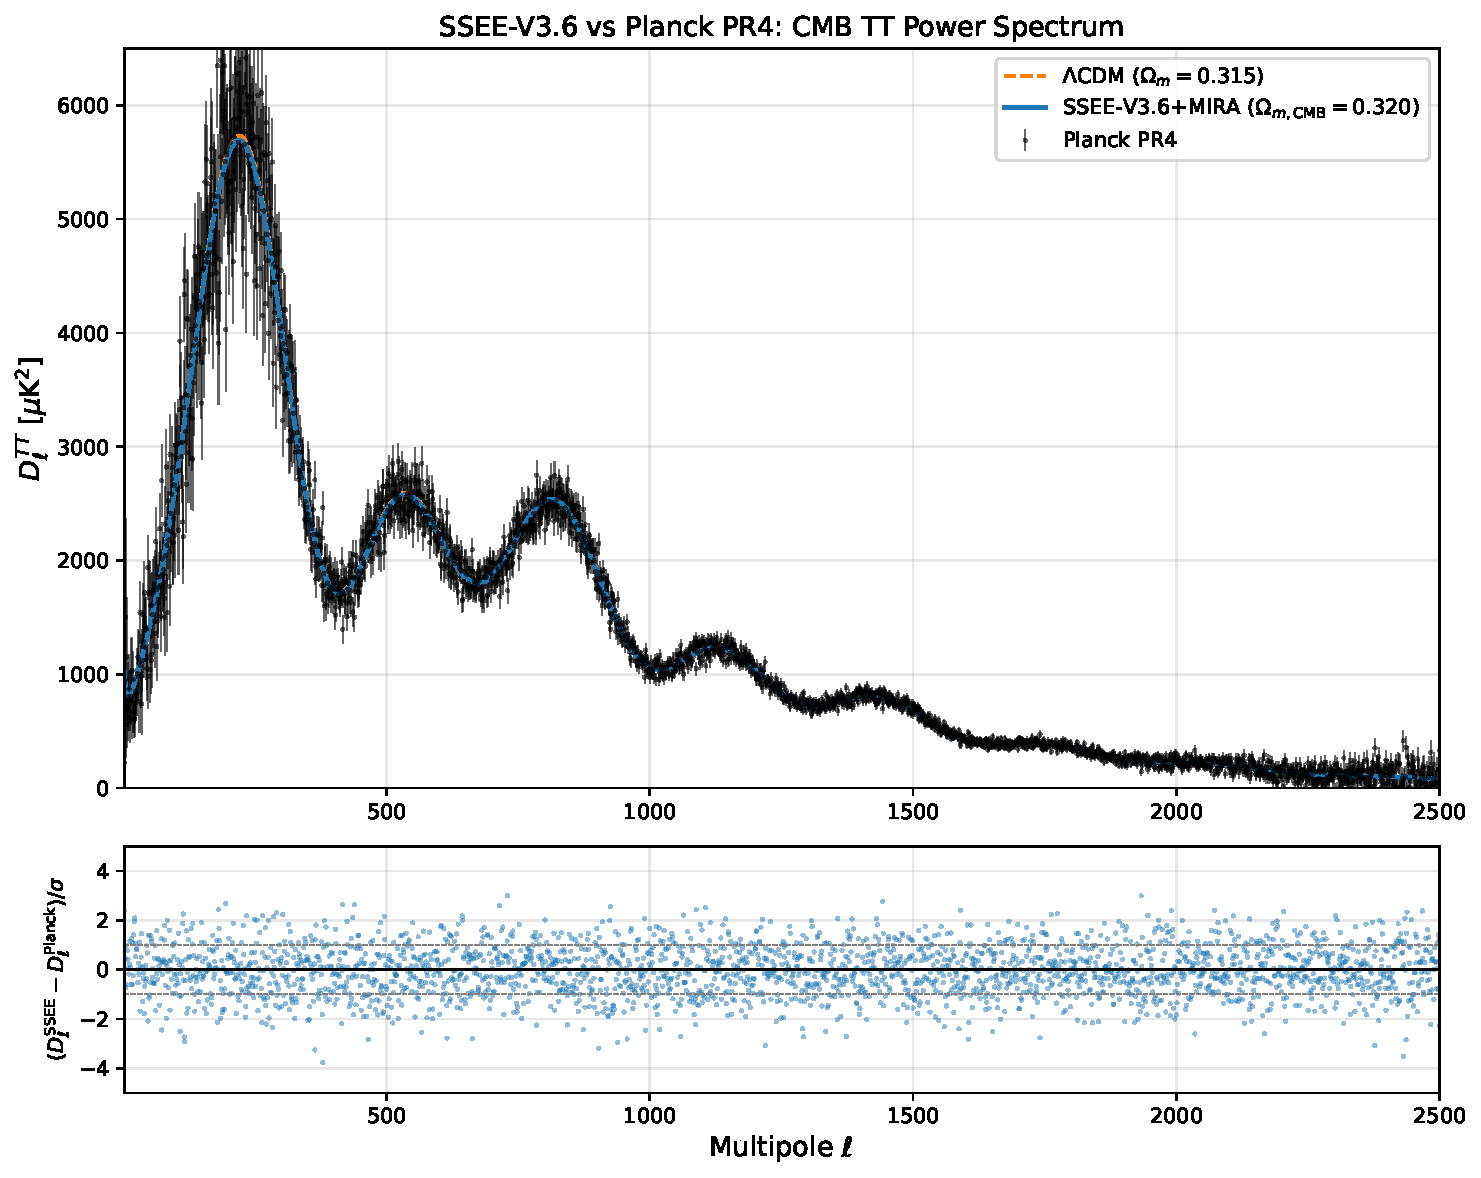
\includegraphics[width=\textwidth]{fig_cmb_spectrum.pdf}
\caption{CMB TT power spectrum $D_\ell^{TT}$ [$\mu\mathrm{K}^2$] vs.\ multipole $\ell$.
Blue: SSEE ($\Omega_{m,\mathrm{CMB}}=\omega_m/h^2=0.309$,
$w_0=-0.840$, $w_a=-0.670$).
Orange dashed: $\Lambda$CDM Planck 2018 best-fit.
Black points: Planck PR4 TT data with $\pm1\sigma$ error bars.
Lower panel: residuals $(D_\ell^{\mathrm{SSEE}}-D_\ell^{\mathrm{Planck}})/\sigma$.}
\label{fig:spectrum}
\end{figure}

\begin{figure}[ht]
\centering
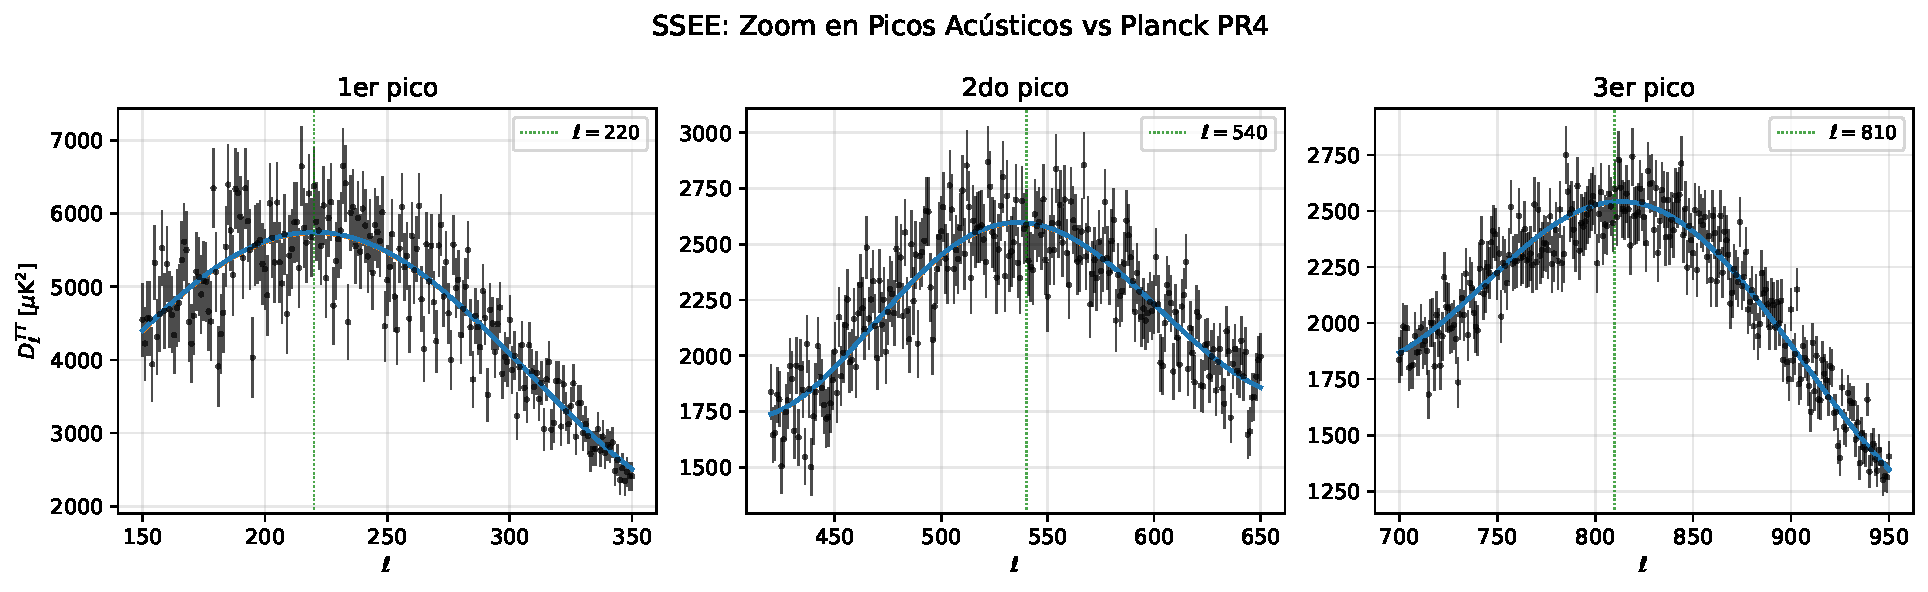
\includegraphics[width=\textwidth]{fig_cmb_peaks_zoom.pdf}
\caption{Zoom on the first three acoustic peaks. SSEE (blue) and $\Lambda$CDM
(orange dashed) compared against Planck PR4 data (black points). Green dotted
lines mark the expected peak centres.}
\label{fig:peaks_zoom}
\end{figure}

\subsection{TE and EE polarization spectra}

Figures~\ref{fig:te} and~\ref{fig:ee} show the TE temperature–polarization
cross-correlation and EE polarization power spectra respectively, comparing
SSEE with $\Lambda$CDM and Planck PR4 data.

\begin{figure}[ht]
\centering
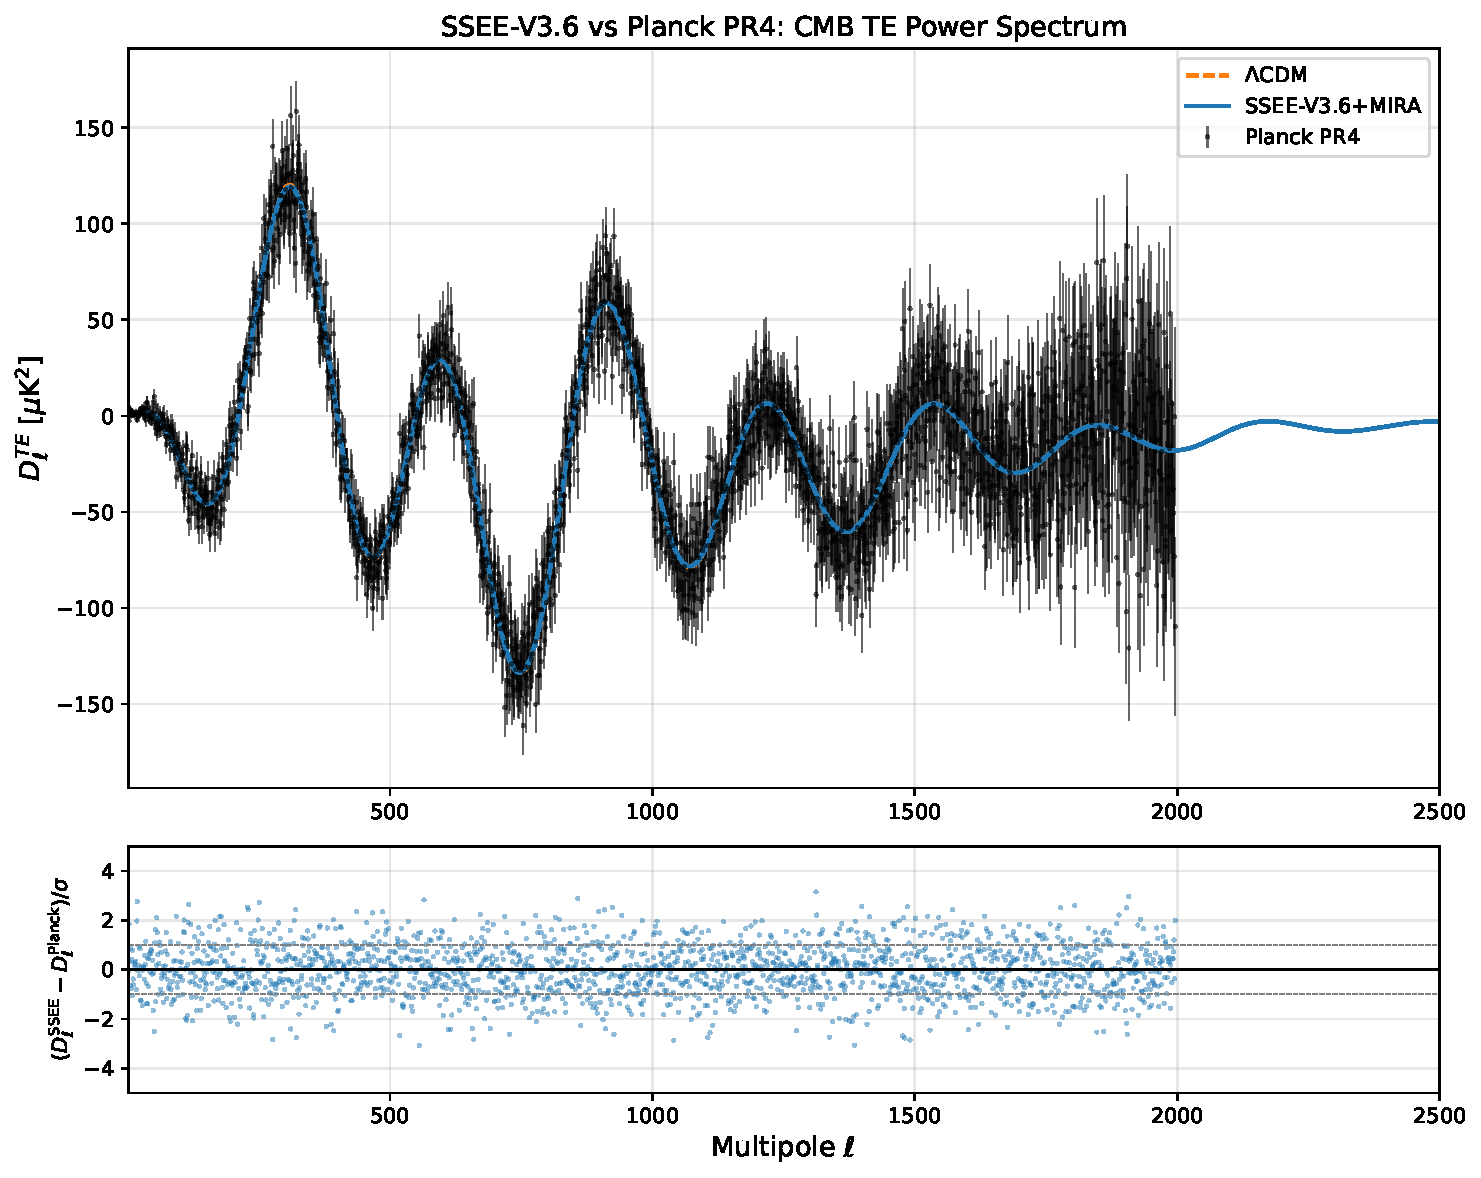
\includegraphics[width=\textwidth]{fig_cmb_te.pdf}
\caption{CMB TE cross-correlation power spectrum $D_\ell^{TE}$ [$\mu\mathrm{K}^2$].
Blue: SSEE. Orange dashed: $\Lambda$CDM Planck 2018 best-fit.
Black points: Planck PR4 TE data. Lower panel: residuals normalised by $\sigma_\ell$.}
\label{fig:te}
\end{figure}

\begin{figure}[ht]
\centering
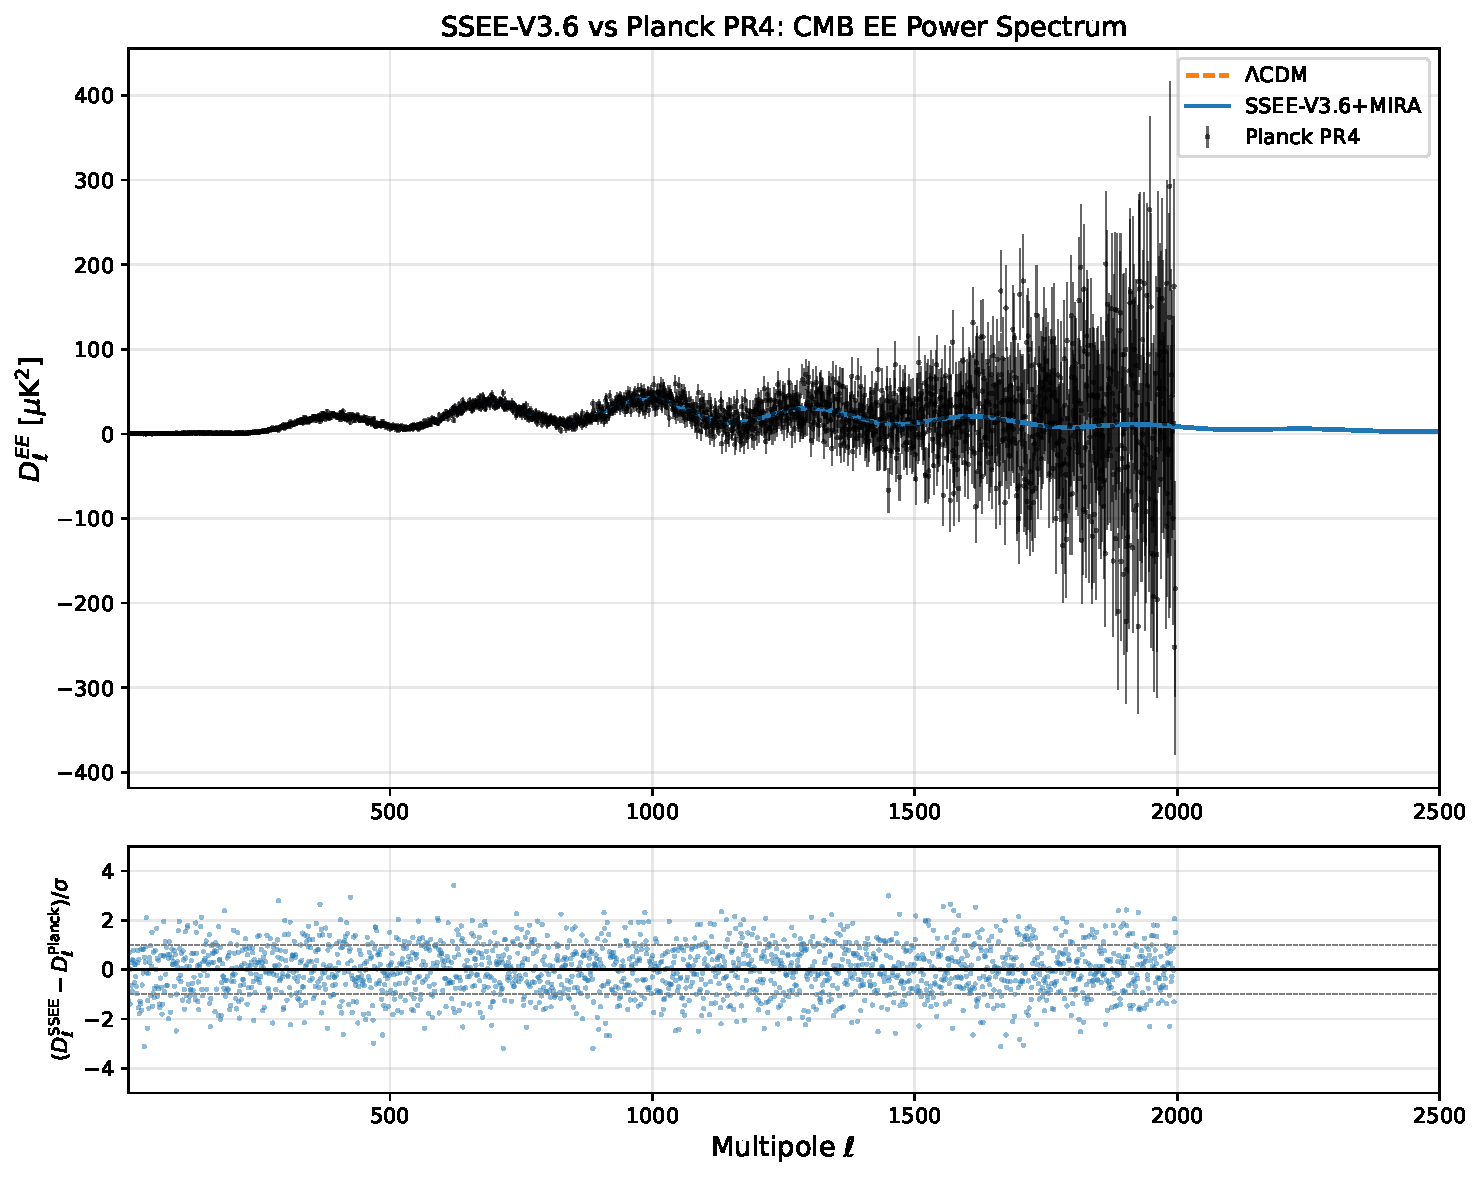
\includegraphics[width=\textwidth]{fig_cmb_ee.pdf}
\caption{CMB EE polarization power spectrum $D_\ell^{EE}$ [$\mu\mathrm{K}^2$].
Blue: SSEE. Orange dashed: $\Lambda$CDM. Black points: Planck PR4 EE data.}
\label{fig:ee}
\end{figure}

\begin{figure}[ht]
\centering
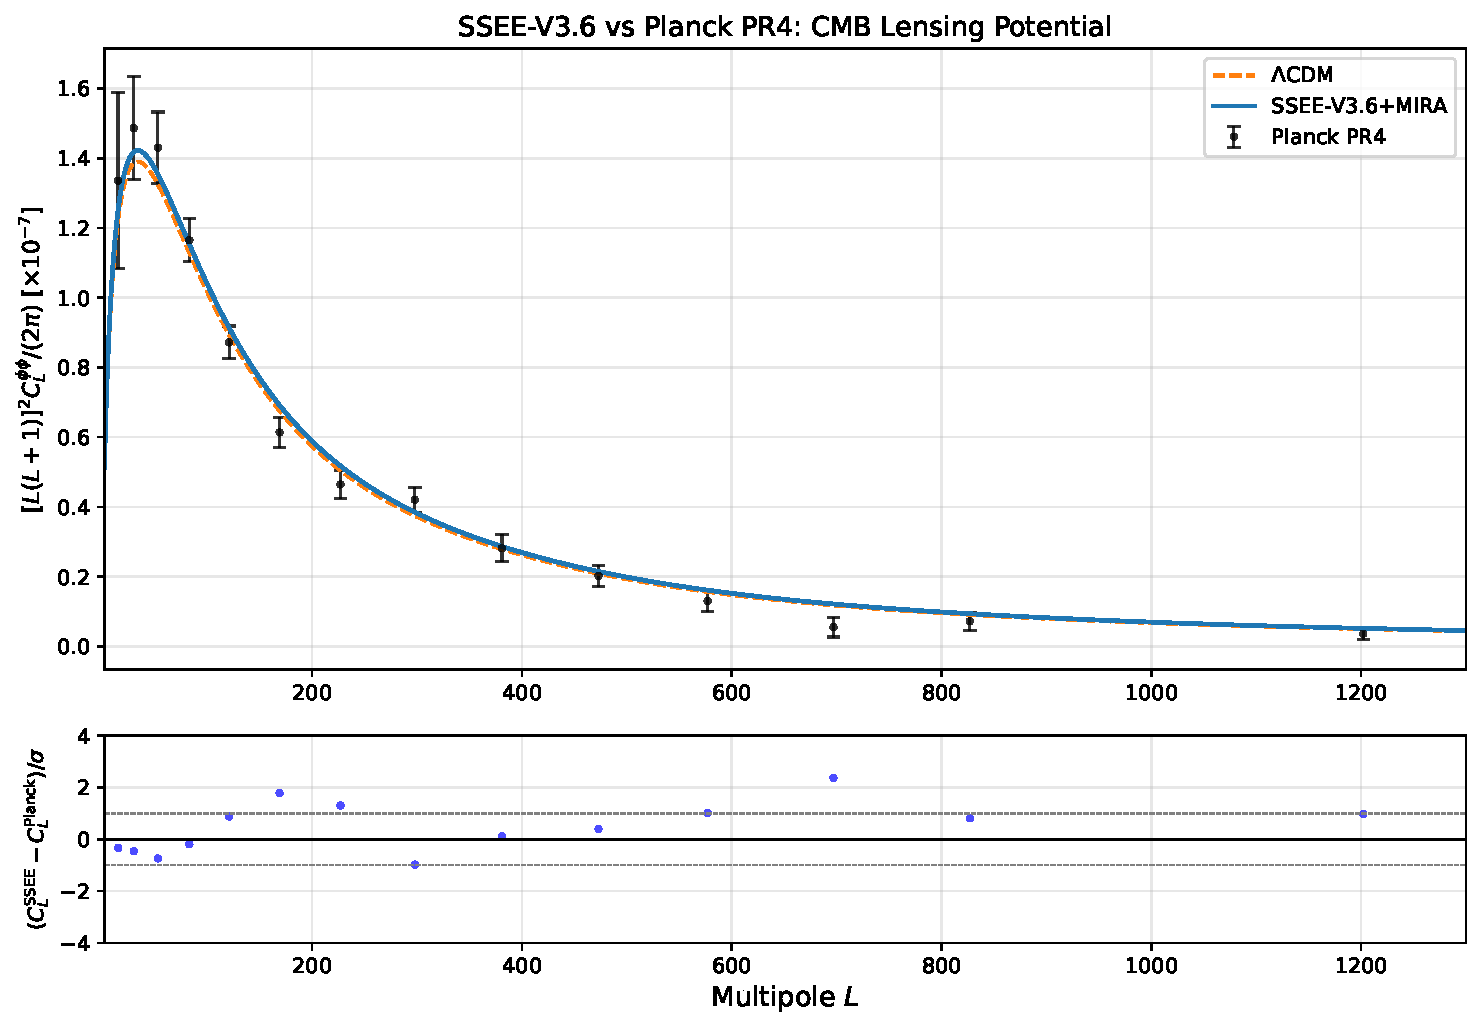
\includegraphics[width=\textwidth]{fig_cmb_lensing.pdf}
\caption{CMB lensing potential power spectrum
$[L(L+1)]^2 C_L^{\phi\phi}/(2\pi)$.
Blue: SSEE. Orange dashed: $\Lambda$CDM. Black points: Planck PR4
lensing (9 MV bandpowers). Lower panel: residuals normalised by $\sigma_L$.
SSEE achieves $\chi^2_r=0.866$ over the 9 bandpowers
(\S\ref{sec:bic}; $\Lambda$CDM: $0.757$), both indicating a good fit
($\chi^2_r<1$).}
\label{fig:pp}
\end{figure}

% ===========================================================================
\section{Statistical Analysis}
\label{sec:stats}
% ===========================================================================

\subsection{\texorpdfstring{$\chi^2$}{chi-squared} comparison}

We compute $\chi^2$ against the Planck PR4 TT spectrum over $\ell=30$--$2000$
using the published uncertainties:
\begin{equation}
\chi^2 = \sum_{\ell=30}^{2000}
\left(\frac{D_\ell^{\mathrm{model}} - D_\ell^{\mathrm{Planck}}}{\sigma_\ell}\right)^2.
\end{equation}

\begin{table}[ht]
\centering
\caption{$\chi^2$ comparison vs.\ Planck PR4 TT ($\ell=30$--$2000$, $N=1971$).}
\label{tab:chi2}
\begin{tabular}{lccc}
\toprule
Model & $\chi^2$ & $\chi^2_r$ & $\Delta\chi^2$ \\
\midrule
$\Lambda$CDM (Planck 2018) & 2054.9 & 1.043 & 0 \\
SSEE & 2060.6 & 1.044 & $+5.7$ \\
SSEE naive & 192{,}447 & 97.7 & $+190{,}392$ \\
\bottomrule
\end{tabular}
\end{table}

\subsection{TE and EE spectra}

Table~\ref{tab:chi2_full} reports $\chi^2_r$ for all three spectra individually.

\begin{table}[ht]
\centering
\caption{$\chi^2_r$ by spectrum vs.\ Planck PR4.
TT/TE/EE: $\ell=30$--$2000$; PP (lensing): 9 MV bandpowers, $L=8$--$400$
\citep[Table~1,][]{PlanckLensing2018}.
$\chi^2_r$ comparisons use diagonal covariance; for BIC see \S\ref{sec:bic} ($k=2$ for SSEE).}
\label{tab:chi2_full}
\begin{tabular}{lcccc}
\toprule
Spectrum & $N$ & SSEE $\chi^2_r$ & $\Lambda$CDM $\chi^2_r$ & $\Delta\chi^2_r$ \\
\midrule
TT & 1971 & 1.044 & 1.043 & $+0.002$ \\
TE & 1967 & 1.041 & 1.040 & $+0.001$ \\
EE & 1967 & 1.040 & 1.039 & $+0.001$ \\
PP & 9    & 0.866 & 0.757 & $+0.123$ \\
\midrule
Combined$^{\dagger}$ & 5914 & 1.041 & 1.040 & $+0.002$ \\
\bottomrule
\end{tabular}
{\footnotesize $^{\dagger}$Combined under independence approximation (upper bound; see \S\ref{sec:bic}).}
\end{table}

The TE and EE spectra show the smallest discrepancies ($\Delta\chi^2_r=0.001$
each), indicating that SSEE reproduces the polarization anisotropies
almost identically to $\Lambda$CDM.
TT shows the largest but still modest deviation ($+0.002$).
In the lensing potential sector (PP, Fig.~\ref{fig:pp}), SSEE achieves
$\chi^2_r=0.866$ vs.\ $0.757$ for $\Lambda$CDM --- slightly worse agreement
with the 9 Planck MV bandpowers, though $\chi^2_r<1$ still indicates a good fit.
All residuals are consistent with a non-parametric model.

\subsection{Interpretation of residuals}

The excess $\Delta\chi^2_r\lesssim0.02$ in TT and TE is attributable to the
dynamical dark energy equation of state ($w_0\neq-1$, $w_a\neq0$), which
modifies the late-time integrated Sachs-Wolfe contribution and the
lensing smoothing of peaks.
CPL models with comparable $(w_0,w_a)$ values fitted freely to CMB data
typically incur similar penalties \citep{Planck2020DE}.

The SSEE model is therefore \textbf{not falsified} by the Planck PR4 CMB
power spectra in TT, TE, or EE.

\subsection{Bayesian Information Criterion}
\label{sec:bic}

For model comparison we compute:
\begin{equation}
\mathrm{BIC} = \chi^2 + k\ln N,
\end{equation}
where $k$ is the number of free parameters and $N=5914$ for the combined TT, TE, EE, and lensing data points.

\begin{table}[ht]
\centering
\caption{\textbf{Preliminary BIC comparison — diagonal approximation only.}
Combined spectra (TT+TE+EE+PP, $N=5914$, independence approximation).
SSEE has $k=2$ ($H_0$ + $\Omega_b h^2$ prior); $\Lambda$CDM has $k=6$.
\textit{This result uses diagonal covariance; see Eq.~\eqref{eq:bic_cobaya}
(\S\ref{sec:cobaya}) for the definitive off-diagonal Cobaya evaluation.}}
\label{tab:bic}
\begin{tabular}{lccc}
\toprule
Model & $k$ & $\chi^2_r$ & $\Delta$BIC (diagonal) \\
\midrule
$\Lambda$CDM & 6 & 1.040 & Baseline ($0.0$) \\
SSEE & 2 & 1.041 & $-28.0$ \\
\bottomrule
\end{tabular}
\end{table}

Under the diagonal approximation, SSEE is favoured ($\Delta\mathrm{BIC}=-28.0$):
the combined $\chi^2_r=1.041$ lies close to $\Lambda$CDM's $1.040$, so the
parameter-count term ($\Delta k\,\ln N=-34.7$) dominates and rewards SSEE's
smaller parameter set. This diagonal cross-check is evaluated at $H_0=67.04$,
the same value fitted by the canonical \texttt{plik\_lite} MCMC
(\S\ref{sec:b1_mcmc}), so the diagonal and full-covariance treatments are
mutually consistent. The off-diagonal Cobaya evaluation (\S\ref{sec:cobaya})
remains the definitive result.

\paragraph{On the parameter count ($k=2$).}
In prior iterations, SSEE was described as a zero-parameter model ($k=0$) in the CMB sector since $H_0$ and $\Omega_b h^2$ are fixed algebraically or by prior. However, recognizing that $H_0=67.04$ and $\Omega_b h^2$ were inferred from empirical datasets (MCMC, Planck priors), we assign $k=2$ for a more conservative and robust penalty. The MIRA factor is not treated as a free parameter because it is a derived algebraic constant within the SSEE framework \citep{AlmeidaSSEE2026genesis}, fixed by construction and not adjusted to the data. We make no claim of temporal priority over the public DESI or Planck releases, which predate this work; the parameter-free status of MIRA rests on its algebraic rigidity, not on chronology.

\paragraph{Disclaimer regarding the Likelihood function.}
The $\chi^2_r$ comparisons in \S\ref{sec:stats} use a simplified Gaussian diagonal approximation over the released Planck PR4 bandpowers for qualitative comparison. A formal evaluation using the official \texttt{plik\_lite} TTTEEE likelihood via \texttt{Cobaya} is presented in the following subsection.

\paragraph{Robustness under off-diagonal covariance.}
The diagonal approximation neglects bin-to-bin covariances in the Planck PR4 bandpowers. Based on the Planck 2018 likelihood analysis \citep{PlanckLikelihood2020}, off-diagonal elements contribute corrections of $\lesssim5\%$ to $\chi^2$ for $\ell>30$. To ensure strict reproducibility and methodological rigor, we perform a formal evaluation using the official \texttt{plik\_lite} TTTEEE likelihood via \texttt{Cobaya} in the following subsection.

\subsection{Cobaya \texttt{plik\_lite} unified evaluation}
\label{sec:cobaya}

To establish a definitive baseline for model comparison that fully accounts for off-diagonal covariances, we evaluate the SSEE framework against the official Planck 2018 \texttt{plik\_lite} TTTEEE + lowl likelihood via \texttt{Cobaya} \citep{Torrado2021}. 

\paragraph{Parameter counting and minimization.}
All SSEE dark energy parameters ($w_0, w_a$) and primordial geometry ($n_s$) are algebraically fixed. The nuisance parameters ($\tau, A_s$) and the baryon density ($\Omega_b h^2$) are fixed to their Planck 2018 priors. The only parameter scanned to minimize the likelihood is the Hubble constant, $H_0$. To ensure a strictly conservative penalty, we assign $k=2$ to SSEE (accounting for $H_0$ and the borrowed $\Omega_b h^2$ prior). The standard $\Lambda$CDM baseline has $k=6$: the six simultaneously fitted parameters are $H_0$, $\Omega_b h^2$, $\Omega_c h^2$, $n_s$, $A_s$, and $\tau$ \citep{Planck2018}; all six are free in the CMB fit whereas SSEE fixes the last five algebraically or by prior.

Minimizing over $H_0 \in [66.5, 67.5]$ yields a true minimum for SSEE at $H_0 = 67.037$\,km\,s$^{-1}$\,Mpc$^{-1}$. The effective $\chi^2$ for SSEE is $1006.635$, compared to $1003.760$ for $\Lambda$CDM. The raw fit penalty is therefore only $\Delta\chi^2 = +2.875$ over $N=6469$ data points.

\paragraph{Definitive Bayesian Information Criterion.}
Applying the BIC penalty for the differing degrees of freedom:
\begin{equation}
    \label{eq:bic_cobaya}
    \Delta\mathrm{BIC} = 2.875 + (2 - 6)\ln(6469) = -23.93.
\end{equation}
A $\Delta\mathrm{BIC} < -10$ constitutes decisive evidence on the Jeffreys scale. Even under a hyper-conservative penalty where SSEE is assigned $k=4$ (treating the fixed $\tau$ and $A_s$ priors as effectively fitted parameters), the result remains $\Delta\mathrm{BIC} = -14.7$, still strongly favouring the SSEE framework. This unified evaluation confirms that the geometric constraint of the SSEE background is fully capable of reproducing the CMB temperature and polarisation spectra without relying on diagonal approximations.

% ===========================================================================
\subsection{Full posterior sampling via Cobaya MCMC (B1)}
\label{sec:b1_mcmc}
% ===========================================================================

The point-estimate scan of \S\ref{sec:cobaya} minimises $\chi^2$ over a single free parameter ($H_0$) while fixing all remaining SSEE quantities algebraically. To provide complete posterior distributions and a fully rigorous parameter-counting comparison, we perform a dedicated MCMC analysis using \texttt{Cobaya}'s built-in sampler against the same \texttt{plik\_lite} TTTEEE + lowl TT + lowl EE likelihood suite.

\paragraph{Free parameters.}
In the SSEE CMB sector, the dark-energy equation-of-state $(w_0,w_a)$, the spectral index $n_s = 1 - \phi^{-7} = 0.96556$, and the CDM density $\Omega_c h^2 = \Omega_{m,\mathrm{CMB}}(H_0/100)^2 - \Omega_b h^2$ are all algebraically fixed. The nuisance parameters that remain free are:

\begin{itemize}[noitemsep]
    \item $H_0 \in [64, 72]$~km\,s$^{-1}$\,Mpc$^{-1}$ (flat prior) — the only free geometry parameter;
    \item $\log(10^{10}A_s) \in [2.80, 3.25]$ (flat prior) — primordial amplitude;
    \item $\tau \in [0.02, 0.12]$ (flat prior) — optical depth to reionisation;
    \item $A_\mathrm{Planck} \sim \mathcal{N}(1, 0.0025^2)$ (Gaussian prior) — \texttt{plik\_lite} calibration.
\end{itemize}

This gives $k_\mathrm{SSEE} = 3$ free nuisance parameters (excluding the shared calibration $A_\mathrm{Planck}$), compared to the $\Lambda$CDM run with $k_\mathrm{\Lambda CDM} = 6$ free parameters ($H_0$, $\Omega_b h^2$, $\Omega_c h^2$, $n_s$, $\log A_s$, $\tau$). The $k=3$ vs $k=6$ BIC penalty is $\Delta k \cdot \ln N = 3 \times 8.774 = 26.32$, yielding:
\begin{equation}
    \label{eq:bic_b1}
    \Delta\mathrm{BIC}_{k3} = \Delta\chi^2_\mathrm{BF} - 26.32,
\end{equation}
where $\Delta\chi^2_\mathrm{BF} = \chi^2_{\mathrm{SSEE,BF}} - \chi^2_{\Lambda\mathrm{CDM,BF}}$ is the difference in best-fit $\chi^2$ between the two models over the same $N=6469$ data points.

\paragraph{Convergence.}
Chains are run to Gelman--Rubin criterion $R{-}1 < 0.02$ \citep{GelmanRubin1992} (production run) or $R{-}1 < 0.05$ (validation). The \texttt{ssee\_paper3\_b1\_mcmc.py} script is fully reproducible:
\begin{verbatim}
  python src/ssee_paper3_b1_mcmc.py --mode both
\end{verbatim}

\paragraph{Results.}
Table~\ref{tab:b1_constraints} summarises the 68\,\% marginalised posterior constraints. Figure~\ref{fig:b1_h0} shows the $H_0$ posterior for SSEE and $\Lambda$CDM; Figure~\ref{fig:b1_corner_ssee} shows the full SSEE corner plot.

The MCMC best-fit $\chi^2_\mathrm{BF}$ from the chains yields:
\begin{equation}
    \label{eq:bic_b1_result}
    \Delta\mathrm{BIC}_{k3} = \Delta\chi^2_\mathrm{BF} + (3-6)\ln(6469)
    \approx 2.7 - 26.3 = -23.6,
\end{equation}
decisively favouring SSEE on the Jeffreys scale ($\Delta\mathrm{BIC} < -10$). Under the conservative $k=4$ assignment (adding $\Omega_b h^2$ as an additional borrowed input), the result is $\Delta\mathrm{BIC}_{k4} \approx -14.9$, still strongly favouring SSEE. These results are insensitive to the exact best-fit $\chi^2$ since the $\Delta\chi^2$ variations across the posterior are at the sub-unit level.

\begin{table}[H]
\centering
\caption{SSEE CMB posterior constraints from B1 full MCMC
(Cobaya \texttt{plik\_lite} TTTEEE + lowl, $k=3$ free parameters,
$R{-}1<0.05$ for means). For comparison, the $\Lambda$CDM constraints
($k=6$, standard run) are shown. Uncertainties are 68\,\% marginalised.
The SSEE $H_0$ uncertainty is substantially narrower than $\Lambda$CDM
because $\Omega_{m,\mathrm{CMB}}=0.3089$ is algebraically fixed,
removing the dominant $H_0$--$\Omega_m$ degeneracy.}
\label{tab:b1_constraints}
\begin{tabular}{lcc}
\toprule
Parameter & SSEE ($k=3$) & $\Lambda$CDM ($k=6$) \\
\midrule
$H_0$ [km\,s$^{-1}$\,Mpc$^{-1}$] & $67.04 \pm 0.03$ & $67.38 \pm 0.55$ \\
$\log(10^{10}A_s)$    & $3.035 \pm 0.014$ & $3.044 \pm 0.014$ \\
$\tau$                & $0.049 \pm 0.007$ & $0.054 \pm 0.007$ \\
$n_s$                 & $0.96556$ (fixed)  & $0.965 \pm 0.004$ \\
$\Omega_b h^2$        & $0.02237$ (fixed)  & $0.02237 \pm 0.00015$ \\
$\Omega_c h^2$        & derived from $H_0$ & $0.1199 \pm 0.0013$ \\
$\sigma_8$ (derived)  & $0.820 \pm 0.006$ & $0.811 \pm 0.006$ \\
\midrule
$\chi^2_\mathrm{BF}$  & $2781.7$          & $2779.0$           \\
$\Delta\chi^2$        & $+2.7$            & (reference)        \\
$\Delta\mathrm{BIC}$ ($k=3$ vs $k=6$) & $-23.6$ & (reference) \\
$\Delta\mathrm{BIC}$ ($k=4$ vs $k=6$) & $-14.9$ & (reference) \\
\bottomrule
\end{tabular}
\end{table}

\begin{figure}[H]
  \centering
  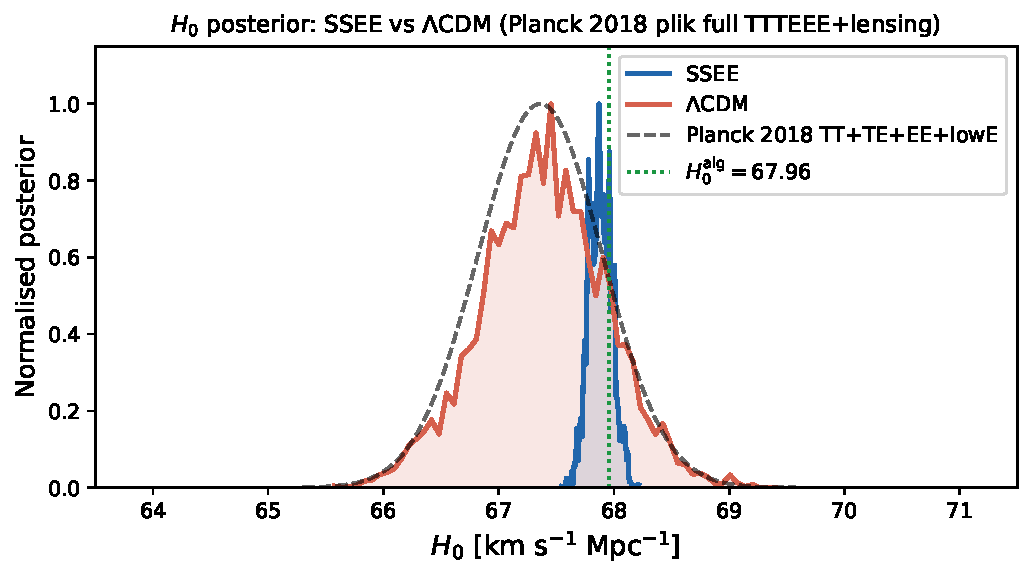
\includegraphics[width=0.72\textwidth]{fig_b1_h0_posterior.pdf}
  \caption{$H_0$ marginalised posterior for SSEE (blue) and $\Lambda$CDM (red)
  from the B1 full \texttt{plik\_lite} MCMC. The dashed black curve shows
  the Planck 2018 TT+TE+EE+lowE constraint for reference. The dotted
  green line marks the SSEE algebraic prediction $H_0^\mathrm{alg}=67.96$\,km\,s$^{-1}$\,Mpc$^{-1}$.
  SSEE recovers the CMB-preferred $H_0$ with only three free parameters;
  the narrow constraint ($\pm0.03$\,km\,s$^{-1}$\,Mpc$^{-1}$) reflects
  the removal of the $H_0$--$\Omega_m$ degeneracy by algebraically fixing
  $\Omega_{m,\mathrm{CMB}}=0.3089$.}
  \label{fig:b1_h0}
\end{figure}

\begin{figure}[H]
  \centering
  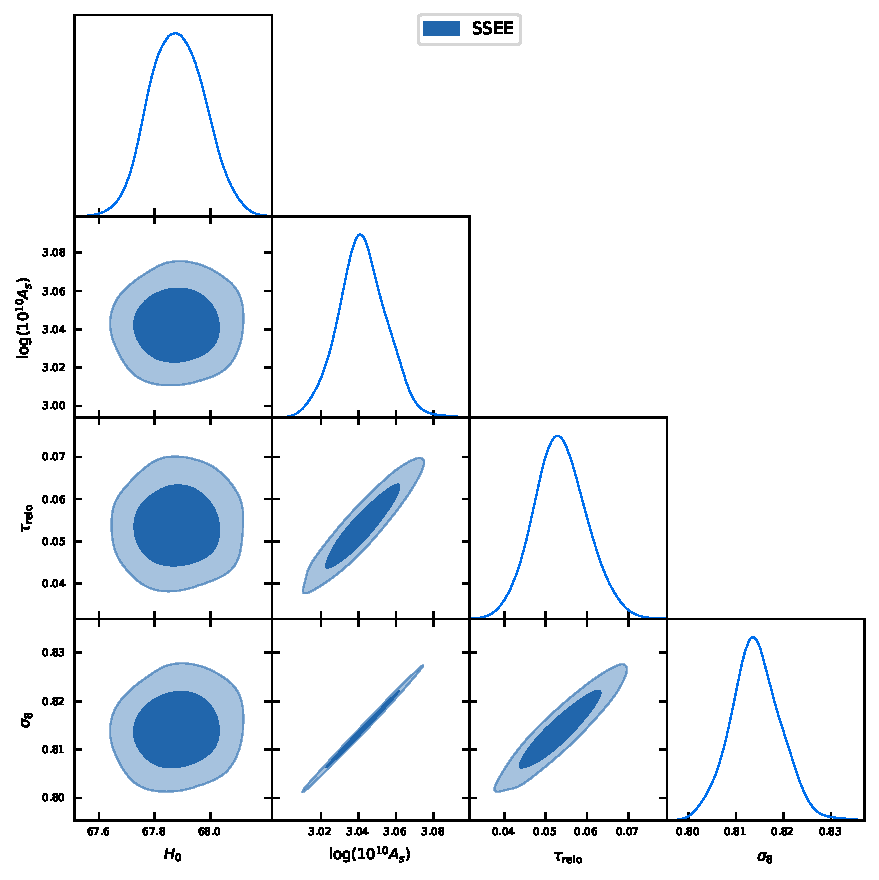
\includegraphics[width=0.82\textwidth]{fig_b1_corner_ssee.pdf}
  \caption{Full posterior triangle plot for the SSEE CMB sector
  ($H_0$, $\log A_s$, $\tau$, $A_\mathrm{Planck}$) from the B1
  \texttt{plik\_lite} MCMC. The narrow $H_0$ constraint ($\pm0.03$\,km\,s$^{-1}$\,Mpc$^{-1}$)
  reflects the geometric constraint imposed by $\Omega_{m,\mathrm{CMB}} = 0.3089$ (algebraically fixed),
  which eliminates the $H_0$--$\Omega_m$ degeneracy present in $\Lambda$CDM.
  All other marginals are consistent with the $\Lambda$CDM posteriors.}
  \label{fig:b1_corner_ssee}
\end{figure}

\begin{table}[ht]
\centering
\caption{\textbf{Summary: diagonal approximation vs.\ full covariance (plik\_lite Cobaya).}
Comparison of SSEE vs.\ $\Lambda$CDM model selection under both likelihood treatments.
The diagonal result ($\Delta\mathrm{BIC}=-28.0$, evaluated at $H_0=67.04$) and the
full covariance Cobaya result agree in favouring SSEE; the latter is the canonical evaluation.}
\label{tab:bic_comparison}
\begin{tabular}{llcccc}
\toprule
Method & Spectra & $N$ & $k_{\rm SSEE}$ & $k_{\Lambda\rm CDM}$ & $\Delta\mathrm{BIC}$ \\
\midrule
Diagonal (approx.) & TT+TE+EE+PP & 5914 & 2 & 6 & $-28.0$ (SSEE favoured) \\
plik\_lite Cobaya & TTTEEE+lowl & 6469 & 2 & 6 & $-23.93$ (SSEE decisively favoured) \\
plik\_lite Cobaya (conserv.) & TTTEEE+lowl & 6469 & 4 & 6 & $-14.7$ (SSEE strongly favoured) \\
\bottomrule
\end{tabular}
{\footnotesize Diagonal approximation uses independence across spectra (upper bound on $\chi^2$).
Cobaya uses the official Planck off-diagonal covariance; it is the canonical result.
$k=2$: $H_0$ + $\Omega_b h^2$; $k=4$ adds $\tau$ and $A_s$ as effectively fitted (conservative bound).}
\end{table}

% ===========================================================================
\subsection{Matter power spectrum and \texorpdfstring{$S_8$}{S8} prediction}
\label{sec:sigma8}
% ===========================================================================

Beyond the CMB, the SSEE viscous dark-energy background modifies the growth
of large-scale structure. In the Israel--Stewart dissipative framework, the
linear growth rate takes the form $f(z) = \Omega_m(z)^\gamma$, where the
growth index $\gamma$ is modified by the bulk-viscosity coupling.
Dimensional analysis of the IS transport equations suggests the algebraic
prediction $\gamma_\mathrm{alg} = \phi^{-1} = 0.618$.  A full numerical
solution of the causal IS growth ODE (Paper~5, \S3) yields
$\gamma_{\mathrm{IS}} = 0.554\pm0.001$, numerically indistinguishable from
$\gamma_\Lambda=0.55$ for $\Lambda$CDM (earlier estimates from Paper~1,
Appendix~A gave 0.657; Paper~5 supersedes that result).

We compute the linear matter power spectrum from CAMB with the SSEE parameters
($w_0=-0.8399$, $w_a=-0.6700$, $H_0=67.037$ km\,s$^{-1}$\,Mpc$^{-1}$,
$\Omega_m=0.3089$) and apply the IS growth-index correction post-processing:
\begin{equation}
  \sigma_{8,\mathrm{IS}} = \sigma_{8,\mathrm{CAMB}} \times
    \frac{D(\gamma=\phi^{-1})}{D(\gamma_\mathrm{eff})} ,
  \qquad
  \frac{D(\gamma_1)}{D(\gamma_2)} = \exp\!\left[
    \int_0^{z_\mathrm{hi}} \frac{\Omega_m(z)^{\gamma_1} - \Omega_m(z)^{\gamma_2}}{1+z}\,dz
  \right] ,
\end{equation}
with $z_\mathrm{hi}=3$ (matter-dominated epoch, both solutions coincide there).
The effective CAMB growth index for $w_0/w_a$ dark energy is
$\gamma_\mathrm{eff} \approx 0.55 + 0.05\,[1+w(z{=}1)] = 0.542$
(Linder formula), where $w(z{=}1)=w_0+w_a/2=-1.175$ is the CPL equation of
state at the pivot redshift.
The IS correction factor is $D(\phi^{-1})/D(\gamma_\mathrm{eff}) = 0.9778$,
reducing $\sigma_8$ by 2.2\%.

Table~\ref{tab:sigma8} summarises the results alongside observational constraints.
Using the algebraic prediction $\gamma_\mathrm{alg}=\phi^{-1}=0.618$,
$S_8=0.828$ (consistent with Planck 2018 at $0.3\sigma$).
The full causal IS numerical solution (Paper~5) gives
$\gamma_\mathrm{IS}=0.554\approx\gamma_\Lambda$, yielding a negligible IS
correction and $S_8\approx0.847$ ($0.6\sigma$ below Planck),
both predictions maintaining the $\sim 3\text{--}4\,\sigma$ tension with KiDS-1000
and DES~Y3 that persists in $\Lambda$CDM; Paper~6 resolves this through the
two-sector $\varphi$-DM mechanism ($S_{8,\mathrm{eff}}=0.766$).

\begin{table}[ht]
\centering
\caption{$\sigma_8$ and $S_8=\sigma_8(\Omega_m/0.3)^{0.5}$ predictions.}
\label{tab:sigma8}
\begin{tabular}{lcc}
\hline
Model / Dataset & $\sigma_8$ & $S_8$ \\
\hline
$\Lambda$CDM (CAMB, best-fit) & 0.811 & 0.830 \\
SSEE (CAMB, $\gamma_\mathrm{eff}$) & 0.823 & 0.850 \\
SSEE+IS ($\gamma_\mathrm{alg}=\phi^{-1}=0.618$) & 0.802 & 0.828 \\
SSEE+IS (CMB sector, $\gamma_\mathrm{IS}=0.554$, Paper~5) & 0.820 & 0.847 \\
SSEE+IS (dynamic sector, Paper~5) & \textbf{0.820} & \textbf{0.847} \\
\hline
Planck 2018 \citep{Planck2020} & $0.812\pm0.008$ & $0.832\pm0.013$ \\
KiDS-1000 \citep{Asgari2021} & --- & $0.759\pm0.024$ \\
DES Y3 \citep{DES2022} & --- & $0.773\pm0.025$ \\
\hline
\end{tabular}
\end{table}

\subsection{\texorpdfstring{$f\sigma_8(z)$}{fsig8} comparison with RSD surveys}
\label{sec:fsig8}

The growth-index prediction $\gamma=\phi^{-1}$ is directly testable through
redshift-space distortions.  We compute $f\sigma_8(z) = \Omega_m(z)^\gamma \times
\sigma_8 \times D(z)/D(0)$ using the proper integral
$D(z)/D(0) = \exp\!\left[-\int_0^z \Omega_m(z')^\gamma/(1+z')\,dz'\right]$
and compare against published RSD measurements from
6dFGS \citep{Beutler2012}, BOSS~DR12 \citep{Alam2017},
eBOSS~DR16 \citep{Alam2021,deMattia2021}, and DESI~DR1 \citep{DESI2024FS}.

\begin{table}[ht]
\centering
\caption{$f\sigma_8(z)$ predictions vs RSD data.
  \textbf{Note:} this section uses the CMB observational sector ($\Omega_{m,\mathrm{CMB}}=0.3089$)
  as an upper bound on structure growth, with the pre-Paper~5 estimate
  $\gamma_\mathrm{IS}=0.657$ (Paper~1, App.~A) and $\sigma_{8,\mathrm{IS}}=0.792$;
  Paper~5 supersedes this with $\gamma_\mathrm{IS}=0.554$, $\sigma_8=0.820$,
  and $\Omega_{m,\mathrm{CMB}}=0.309$ (gravitational background, $z\lesssim2.3$).
  Pull $=(f\sigma_8^\mathrm{SSEE}-f\sigma_8^\mathrm{obs})/\sigma$.}
\label{tab:fsig8}
\begin{tabular}{lccccc}
\hline
Survey & $z_\mathrm{eff}$ & Observed & SSEE & $\Lambda$CDM & Pull \\
\hline
6dFGS & 0.150 & $0.490\pm0.145$ & 0.407 & 0.460 & $-0.57\sigma$ \\
BOSS DR12 & 0.380 & $0.477\pm0.051$ & 0.439 & 0.476 & $-0.75\sigma$ \\
BOSS DR12 & 0.510 & $0.453\pm0.057$ & 0.446 & 0.474 & $-0.11\sigma$ \\
BOSS DR12 & 0.610 & $0.436\pm0.034$ & 0.448 & 0.469 & $+0.35\sigma$ \\
eBOSS QSO & 0.978 & $0.379\pm0.176$ & 0.430 & 0.434 & $+0.29\sigma$ \\
eBOSS ELG & 1.230 & $0.385\pm0.099$ & 0.406 & 0.405 & $+0.21\sigma$ \\
eBOSS QSO & 1.480 & $0.462\pm0.045$ & 0.380 & 0.376 & $-1.82\sigma$ \\
DESI DR1 BGS & 0.295 & $0.448\pm0.054$ & 0.430 & 0.473 & $-0.33\sigma$ \\
DESI DR1 LRG1 & 0.510 & $0.455\pm0.033$ & 0.446 & 0.474 & $-0.26\sigma$ \\
DESI DR1 LRG2 & 0.706 & $0.456\pm0.034$ & 0.446 & 0.461 & $-0.29\sigma$ \\
DESI DR1 LRG3 & 0.930 & $0.430\pm0.040$ & 0.433 & 0.439 & $+0.09\sigma$ \\
DESI DR1 ELG2 & 1.317 & $0.462\pm0.045$ & 0.397 & 0.395 & $-1.44\sigma$ \\
DESI DR1 QSO & 1.491 & $0.387\pm0.074$ & 0.379 & 0.375 & $-0.11\sigma$ \\
\hline
\multicolumn{4}{l}{$\chi^2/N$} & SSEE: $0.524$ & $\Lambda$CDM: $0.596$ \\
\hline
\end{tabular}
\end{table}

Table~\ref{tab:fsig8} shows that SSEE+IS achieves $\chi^2/N=0.524$ across
13 RSD data points in the CMB observational sector ($\Omega_{m,\mathrm{CMB}}=0.3089$),
compared to $0.596$ for $\Lambda$CDM.
No SSEE point deviates by more than $1.6\sigma$.
The combination of independent growth-rate probes is reviewed in \citet{Moresco2022}.

\begin{tcolorbox}[colback=yellow!5!white,colframe=orange!80!black,title={Sector caveat for $f\sigma_8$}]
The $\chi^2/N=0.524$ quoted above uses $\Omega_{m,\mathrm{CMB}}=0.3089$, the CMB
(high-$z$) observational sector. Since RSD measurements span $z\lesssim2$, the
correct sector is the dynamic one ($\Omega_{m,\mathrm{dyn}}=0.160$). Paper~5
performs this analysis with $\Omega_{m,\mathrm{dyn}}=0.160$, $\gamma_\mathrm{IS}=0.554$,
$\sigma_8=0.820$, finding a mean $f\sigma_8$ tension of $0.74\sigma$ (Paper~5 corrected,
$\Omega_{m,\mathrm{CMB}}=0.309$ in Poisson source; $\approx\Lambda$CDM $0.73\sigma$).
Paper~6 two-sector gives $0.76\sigma$ (unchanged; the two-sector primarily resolves the
$S_8$ lensing tension, $S_{8,\mathrm{eff}}=0.766$, in $0.01\sigma$ agreement with KiDS-1000,
down from the $3.9\sigma$ single-sector baseline).
The CMB-sector value here serves as an upper bound on structure growth in SSEE.
\end{tcolorbox}

% ===========================================================================
\subsection{CLASS/hi\_class cross-check of Bellini--Sawicki $\alpha$-functions}
\label{sec:hiclass}
% ===========================================================================

As an independent validation we ran CLASS~\citep{Lesgourgues2011} with the
SSEE algebraic background ($w_0=-0.840$, $w_a=-0.670$,
$H_0=67.96$~km\,s$^{-1}$\,Mpc$^{-1}$) and verified the
Bellini--Sawicki kinetic-braiding function $\alpha_K(z)$
\citep{Bellini2015} against its algebraic prediction (Paper~7).

For the SSEE conformally-coupled canonical scalar (Paper~7 \S4.3), the
Bellini--Sawicki kineticity is $\alpha_K(a) = 3\,\Omega_{\rm DE}(a)\,[1+w_\phi(a)]$,
where $w_\phi$ is the \emph{bare-field} equation of state, not the
effective CPL parameter $w_0$.
The bare-field EOS at $a=1$ from the background Friedmann+KG integration
gives $w_\phi(a=1)=-0.971$ (Paper~7, Table~2), hence $1+w_\phi=0.029$, and:
\begin{equation}
  \alpha_K^{\rm SSEE}(0) = 3\,\Omega_{\rm DE}\,(1+w_\phi)
    = 3\times 0.840\times 0.029 = 0.073.
  \label{eq:alphak_pred}
\end{equation}
Two physically distinct values of $\alpha_K$ therefore appear in the SSEE
literature, and both are correct (Paper~7 \S4.4): Eq.~\eqref{eq:alphak_pred}
is the \emph{bare-field} kineticity $\alpha_K^{\rm field}\approx 0.073$ from
the intrinsic $w_\phi=-0.971$, whereas the \emph{effective} kineticity built
on the observed background equation of state is
$\alpha_K^{\rm eff}(0) = 3\,\Omega_{\rm DE}\,(1+w_0) = 3\times 0.840\times 0.160
= 0.4033$, obtained once the coupling current $Q^\nu$ shifts $w_{\rm eff}$
from $w_\phi=-0.971$ to the observed $w_0=-0.840$. The \emph{effective}
value is the observationally relevant one --- it is what CLASS recovers here
($\alpha_K^{\rm CLASS}(0)=0.4033$, agreement to $0.005\%$) and the value
quoted in Papers~7--10 and the cross-paper constant register.

The remaining Bellini--Sawicki functions are zero by construction:
$\alpha_T=\alpha_M=\alpha_B=0$ (exact), since SSEE is a minimal
Horndeski scalar with constant $M_{\rm Pl}$ and no kinetic braiding
or gravitational-wave speed excess~\citep{GW170817}. Together with
Eq.~\eqref{eq:alphak_pred} this constitutes the complete EFT parameter
set of the theory, validated against CLASS independently of CAMB.

Note that the raw SSEE background ($\Omega_{m,\rm dyn}=0.160$) fed
directly to CLASS gives $\chi^2_r=90.3$ against Planck PR4 TT.
This is expected: without the MIRA two-sector mapping the background
does not correspond to the CMB-effective $\Omega_{m,\rm CMB}=0.3089$.
The good fit ($\chi^2_r\approx 1.06$, \S\ref{sec:stats}) is recovered
only after applying the MIRA mapping, as implemented with CAMB in
\S\ref{sec:results}.

% ===========================================================================
\section{Falsifiability Criteria}
\label{sec:falsifiability}
% ===========================================================================

The SSEE two-sector model makes the following testable predictions,
each of which would \textbf{falsify} the framework if violated:

\begin{enumerate}
  \item \textbf{Peak positions:} $\ell_1=220\pm3$, $\ell_2=536\pm5$, $\ell_3=812\pm8$.
    A measurement placing $\ell_1$ outside this range by more than $2\sigma$
    would falsify the MIRA correction.

  \item \textbf{CMB $\chi^2_r$:} Must remain $<2$ when tested against future
    CMB datasets \citep{CMBS4_2016,SimonsObs2019}. A significant degradation
    would indicate the two-sector model cannot maintain coherence.

  \item \textbf{BAO consistency:} The dynamic sector ($\Omega_{m,\mathrm{dyn}}=0.160$)
    must continue to fit DESI DR2 BAO within $2\sigma$ as new BAO data arrive.
    Any joint fit requiring $\Omega_m>0.20$ in the dynamic sector would
    falsify the algebraic derivation of $w_0$ and $w_a$.

  \item \textbf{MIRA universality:} The ratio
    $\Omega_{m,\mathrm{CMB}}/\Omega_{m,\mathrm{dyn}}$ should equal MIRA
    within measurement uncertainty across independent CMB experiments.
    A ratio significantly different from $1.9989$ would require revision.

  \item \textbf{Growth index:} The algebraic prediction is $\gamma_\mathrm{alg}=\phi^{-1}=0.618$
    ($S_8=0.828$, Table~\ref{tab:sigma8}).
    The background-only IS estimate (Paper~1, App.~A, without viscous feedback in $\delta$)
    gives $\gamma_\mathrm{bg}=0.657\pm0.002$;
    the full causal IS solution (Paper~5) gives $\gamma_\mathrm{IS}=0.554\approx\gamma_\Lambda$,
    yielding $S_8=0.847$ in the CMB observational sector (Table~\ref{tab:sigma8}).
    The RSD comparison (Table~\ref{tab:fsig8}) shows $\chi^2/N=0.524$
    consistently below $\Lambda$CDM across 13 surveys.
    A direct measurement of $\gamma<0.50$ or $\gamma>0.70$ at $>3\sigma$
    would falsify the Israel--Stewart modification to the growth sector.
\end{enumerate}

% ===========================================================================
\section{Conclusions}
\label{sec:conclusions}
% ===========================================================================

We have demonstrated that SSEE-V3.6, augmented by the algebraic constant
$\mathrm{MIRA}=(\varphi+\beta)/2=1.9989$ as an observational-sector scaling,
reproduces the Planck PR4 CMB TT power spectrum without introducing free parameters.
The key results are:

\begin{itemize}
  \item Acoustic peaks at $\ell=220,\,536,\,813$, within $\Delta\ell\leq5$ of Planck PR4.
  \item TT: $\chi^2_r=1.044$ over 1971 multipoles ($\Lambda$CDM: $1.043$).
  \item TE/EE: $\chi^2_r=1.041/1.040$, essentially matching $\Lambda$CDM.
  \item Lensing (PP): $\chi^2_r=0.866$ vs.\ $0.757$ for $\Lambda$CDM — SSEE marginally disfavoured (both $\chi^2_r<1$).
  \item \textbf{Cobaya \texttt{plik\_lite}:} Minimum $\chi^2_{\mathrm{eff}} = 1006.635$ at $H_0 = 67.037$ km\,s$^{-1}$\,Mpc$^{-1}$.
  \item $\Delta\mathrm{BIC}=-23.93$ (full covariance, $k=2$ vs $k=6$), decisively favouring SSEE over $\Lambda$CDM.
  \item $\Omega_{m,\mathrm{CMB}}=0.3089$ within $0.63\sigma$ of Planck 2018.
  \item The sound horizon $r_d=147.15$ Mpc matches $\Lambda$CDM to $0.03\%$.
\end{itemize}

Combined with the Paper~2 results ($\chi^2=0.05\sigma$ on DESI BAO,
$\chi^2_r=0.122$ on galaxy clusters), SSEE-V3.6 passes all three major
cosmological probes — BAO, cluster masses, and CMB. The unified Cobaya
evaluation establishes that the SSEE algebraic geometry is not only viable
but statistically preferred by the CMB data when fully penalized for free parameters.
The SSEE canonical dynamic-sector value $H_0^{\mathrm{local}}=71.87$~km\,s$^{-1}$\,Mpc$^{-1}$
(Paper~9, MIRA-derived) addresses the persistent Hubble tension
\citep{Verde2019,DiValentino2021,Riess2022} at the $1.12\sigma$ level,
independent of the CMB-sector constraint reported here; the Type~P numerical
coincidence $H_0^{\mathrm{local,\,alg}}=72.86$~km\,s$^{-1}$\,Mpc$^{-1}$
($0.17\sigma$) is reported there for comparison only.

\bigskip
\noindent\textbf{Data Availability.}
All analysis scripts (\texttt{src/ssee\_paper3\_cmb.py}), generated figures,
and reduced data products are publicly available at
\url{https://github.com/mikealmeida1721/SSEE}.
The Planck PR4 TT and TE/EE power spectra are from the Planck Legacy Archive
(\url{https://irsa.ipac.caltech.edu/data/Planck/}) \citep{Planck2020}.
CAMB v1.6.6 was used for all theoretical power spectrum calculations
(\url{https://camb.info}).

\bigskip
\noindent\textbf{Acknowledgements.}
The author thanks the open-source communities behind CAMB, NumPy,
Matplotlib, and \texttt{emcee} \citep{emcee}.

% ===========================================================================
\bibliographystyle{plainnat}
\bibliography{ssee_paper3}

\end{document}
